\documentclass[12pt,aspectratio=169]{beamer}

\mode<presentation>
{
  \usetheme{Singapore}
 %\setbeamersize{text margin left=.6cm,text margin right=.6cm}
%  \setbeamertemplate{navigation symbols}{} % suppress nav bar
%  \setbeamercovered{transparent}
}
\usefonttheme{professionalfonts}
\usepackage{graphicx}
\usepackage{tikz}
\usepackage{amsmath}
\usepackage{mathpazo}
\usepackage[scaled]{helvet}
\usepackage{xcolor,colortbl}
\usepackage{siunitx}
\usepackage[siunitx]{circuitikz} % to draw circuits!

\sisetup{number-math-rm=\mathnormal}

\title{Class 12: Circuits Analysis}
\subtitle{AP Physics}
\author[TML]{Dr.\ Timothy Leung}
\institute{Olympiads School}
\date{February 2018}

\newcommand{\pic}[2]{\includegraphics[width=#1\textwidth]{#2}}
\newcommand{\mb}[1]{\mathbf{#1}}
\newcommand{\eq}[2]{\vspace{#1}{\Large\begin{displaymath}#2\end{displaymath}}}


\begin{document}

\begin{frame}
  \maketitle
\end{frame}


\section[Intro]{Introduction}

\begin{frame}
  \frametitle{Notice: Tim Will Be Away Next Week}

  \begin{center}
    \fbox{
      \begin{minipage}{.6\textwidth}
        Tim will be away to do a concert in Ottawa next Saturday (February
        17). There will be a supply teacher for next week. Please be kind
        to him! Tim will return to Olympiads on Sunday, February 18,, and will
        resume teaching this class on the 24th (class 14).
      \end{minipage}
    }
  \end{center}
\end{frame}

\begin{frame}
  \frametitle{Files for You to Download}
  Download from the school website:
  \begin{enumerate}
  \item\texttt{12-Circuits\_print.pdf}---The print version of this
    presentation. If you want to print on paper, I recommend printing 4 pages
    per side.
  \item\texttt{13-Homework.pdf}---Homework assignment for this class and next
    class. The file will be posted along Class 13 slides.
  \end{enumerate}

  \vspace{.2in}Please download/print the PDF file before each class. There is
  no point copying notes that are already printed out for you. Instead, take
  notes on things I say that aren't necessarily on the slides.
\end{frame}



\section{Resistors}

\begin{frame}
  \frametitle{Resistors}
%  From last class (and Physics 12), we know that the electric field from a
%  point charge $q$ is given by:
%
%  \eq{-.2in}{\mb{E}=\frac{kq}{r^2}\hat{\mb{r}}}
%  
%  where $\hat{\mb{r}}$ is the outward radial direction from the charge. The
%  total field at a point $P$ from a distribution of charge is found by
%  integrating through the entire volume of the charge:
%
%  \eq{-.2in}{\boxed{\mb{E}=\int_V\frac{kdq}{r^2}\hat{\mb{r}}}}
\end{frame}


\begin{frame}
  \frametitle{Resistors}
%%  \begin{columns}
%%    \column{.3\textwidth}
%%    \pic{1}{thinrod.jpg}
%%    \column{.7\textwidth}
%%    \begin{itemize}
%%    \item A thin rod with length $\ell$, and charge distribution $\lambda$
%%    \item The parallel component $dE_x$ does not contribute, but
%%      perpendicular component $dE_y$ does:
%%
%%      \eq{-.2in}{
%%        dE_y=\frac{k dq}{r^2}\cos\theta
%%        =\frac{k\lambda dx}{r^2}\cos\theta
%%      }
%%    \item We integrate through the 
%%    \end{itemize}
%%  \end{columns}
\end{frame}


\begin{frame}
  \frametitle{Resistors}

\end{frame}


\begin{frame}
  \frametitle{Resistance of a Conductor}
  The resistance of a conductor is proportional to the resistivity $\rho$ and
  its length $L$, and inversely proportional to the cross-sectional area $A$:

  \eq{-.2in}{
    \boxed{R = \rho\frac{L}{A}}
  }

  \begin{center}
    \begin{tabular}{l|c|l}
      \rowcolor{pink}
      \textbf{Quantity} & \textbf{Symbol} & \textbf{SI Unit} \\ \hline
      Resistance           & $R$    & \si{\ohm} (ohms) \\
      Resistivity          & $\rho$ & \si{\ohm.\metre} (ohm metres) \\
      Length of conductor  & $L$    & \si{\metre} (metres) \\
      Cross-sectional area & $A$    & \si{\metre^2} (square metres) \\
    \end{tabular}
  \end{center}
\end{frame}


\begin{frame}
  \frametitle{Resistance of a Conductor}

  \eq{-.2in}{
    \boxed{R = \rho\frac{L}{A}}
  }

  \begin{columns}
    \column{0.5\textwidth}
    \begin{center}
      \begin{tabular}{c|c|c}
        \rowcolor{blue!70!gray}
        {\color{white}Gauge} & 
        {\color{white}Diameter} & 
        {\color{white}$R/L$} \\
        \rowcolor{blue!70!gray}
        & {\color{white}(\si{mm})} & 
        {\color{white}(\SI{e-3}{\ohm/m})}\\ \hline
        0  & \num{9.35} & \num{0.31} \\
        10 & \num{2.59} & \num{2.20} \\
        14 & \num{1.63} & \num{8.54} \\
        18 & \num{1.02} & \num{21.90} \\
        22 & \num{0.64} & \num{51.70} \\
      \end{tabular}
    \end{center}
    \column{0.5\textwidth}
    \begin{center}
      \begin{tabular}{c|c}
        \rowcolor{blue!70!gray}
        {\color{white} Material} & 
        {\color{white} Resistivity $\rho$ (\si{\ohm.m})}\\ \hline
        silver    & \num{1.6e-8} \\
        copper    & \num{1.7e-8} \\
        aluminum  & \num{2.7e-8} \\
        tungsten  & \num{5.6e-8} \\
        Nichrome  & \num{100e-8} \\
        carbon    & \num{3500e-8}\\
        germanium & \num{0.46} \\
        glass     & \num{e10} to \num{e14}\\
      \end{tabular}
    \end{center}
  \end{columns}
\end{frame}



\section{Ohm's Law}

\begin{frame}
  \frametitle{Ohm's Law}

  The electric potential difference $V$ across a ``load'' (resistor) equals the
  product of the current $I$ through the load and the resistance $R$ of the
  load.

  \eq{-.2in}{
    \boxed{V=IR}
  }
  
  \vspace{-.2in}
  \begin{center}
    \begin{tabular}{l|c|l}
      \rowcolor{pink}
      \textbf{Quantity} & \textbf{Symbol} & \textbf{SI Unit} \\ \hline
      Potential difference & $V$    & \si{\volt} (volt) \\
      Current              & $I$    & \si{\ampere} (ampere) \\
      Resistance           & $R$    & \si{\ohm} (ohm) \\
    \end{tabular}
  \end{center}

  A resistor is considered ``ohmic'' if it obeys Ohm's law
\end{frame}


\begin{frame}
  \frametitle{Power Dissipated by a Resistor}

  Power is the rate at which work $W$ is done, and from electrostatics, the
  change in electric potential energy
  $\Delta E_q$ (i.e.\ the work done!) is proportional to the amount of charge
  $q$ and the voltage $V$. This gives a very simple expression for power
  through a resistor:
  
  \eq{-.15in}{
    P=\frac{dW}{dt}=\frac{d(qV)}{dt}=\left(\frac{dq}{dt}\right)V=\boxed{IV}
  }
  \begin{center}
    \begin{tabular}{l|c|l}
      \rowcolor{pink}
      \textbf{Quantity} & \textbf{Symbol} & \textbf{SI Unit} \\ \hline
      Power through a resistor    & $P$ & \si{\watt} (watt) \\
      Current through a resistor  & $I$ & \si{\ampere} (ampere) \\
      Voltage across the resistor & $V$ & \si{\volt} (volt) \\
    \end{tabular}
  \end{center}
\end{frame}

\begin{frame}
  \frametitle{Other Equations for Power}
  When we combine Ohm's Law ($V=IR$) with power equation, we get two additional
  expressions for power through a resistor:

  \eq{-.2in}{
    \boxed{P=\frac{V^2}{R}}\quad\boxed{P=I^2R}
  }
  
  \begin{center}
    \begin{tabular}{l|c|l}
      \rowcolor{pink}
      \textbf{Quantity} & \textbf{Symbol} & \textbf{SI Unit} \\ \hline
      Power      & $P$ & \si{\watt} (watts) \\
      Voltage    & $V$ & \si{\volt} (volts) \\
      Resistance & $R$ & \si{\ohm} (ohms) \\
      Current    & $I$ & \si{\ampere} (amperes) \\
    \end{tabular}
  \end{center}
\end{frame}


\section{Kirchkoff's Laws}

\begin{frame}
  \frametitle{Kirchkoff's Current Law}
  The electric current that flows into any junction in an electric circuit must
  be equal to the current which flows out.

  \vspace{.2in}
  \begin{columns}
    \column{.3\textwidth}
    \begin{center}
      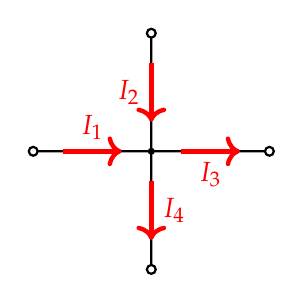
\begin{tikzpicture}[scale=1.5]
        \draw[thick](0,0) to[short,o-] (1,0) to[short,-o] (1,-1);
        \draw[thick](1,1) to[short,o-] (1,0) to[short,-o] (2,0);
        \draw[ultra thick,red,->](.25,0)--(.75,0) node[midway,above]{$I_1$};
        \draw[ultra thick,red,->](1,.75)--(1,.25) node[midway,left]{$I_2$};
        \draw[ultra thick,red,->](1.25,0)--(1.75,0) node[midway,below]{$I_3$};
        \draw[ultra thick,red,->](1,-.25)--(1,-.75) node[midway,right]{$I_4$};
        \fill[black](1,0) circle(0.03);
      \end{tikzpicture}
    \end{center}
    \column{.7\textwidth}
    e.g.\ if there are 4 paths to the junction at the center, with $I_1$ and
    $I_2$ going into the junction, and $I_3$ and $I_4$ coming out, then the
    current law says that

    \eq{-.3in}{I_1+I_2-I_3-I_4=0}
  \end{columns}

  \vspace{.2in}Basically, it means that there cannot be any accumulation of
  charges anywhere in the circuit. The law is a consequence of conservation of
  energy.
\end{frame}


\begin{frame}
  \frametitle{Kirchkoff's Voltage Law}

  The voltage changes around any closed loop in the circuit must sum to zero,
  no matter what path you take through an electric circuit.

  \vspace{.1in}
  \begin{columns}
    \column{.3\textwidth}
    \begin{center}
      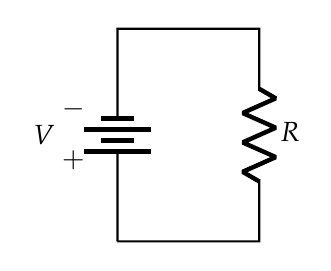
\begin{tikzpicture}[scale=1.8,american voltages]
        \draw[thick](0,0) to[battery=$V$] (0,1.5)--(1,1.5) to[R=$R$] (1,0)--(0,0);
      \end{tikzpicture}
    \end{center}
    \column{.7\textwidth}
    Assume that the current flows clockwise and we draw a clockwise loop, we
    get

    \eq{-.45in}{ V-V_R=0\;\;\rightarrow\;\; V-IR=0}

    \vspace{-.25in}If I incorrectly guess that $I$ flows counterclockwise, I
    will still have a similar expression

    \eq{-.45in}{-V_R-V=0\;\;\rightarrow\;\; -V-IR=0}
  \end{columns}

  \vspace{-.1in}When solving for $I$, we get a negative number, indicating
  that my guess was in the wrong direction.
\end{frame}


\section{Resistors in Circuits}

\begin{frame}
  \frametitle{Resistors in Parallel}
  \begin{columns}
    \column{.32\textwidth}
    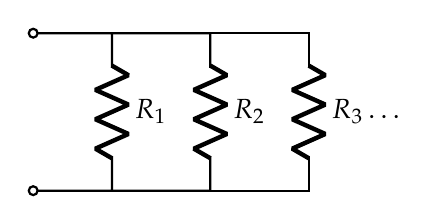
\begin{tikzpicture}
     \draw[thick] (0,2) to[short,o-] (1,2) to[R=$R_1$] (1,0) to[short,-o] (0,0);
     \draw[thick](1,2)  to[short] (2.25,2)to[R=$R_2$] (2.25,0)to[short] (1,0);
     \draw[thick](2.25,2)to[short](3.5,2) to[R=$R_3\ldots$] (3.5,0)
     to[short] (2.25,0);
    \end{tikzpicture}
    \column{.68\textwidth}
    From the current law, we know that the total current is the
    current through all the resistors, which we can rewrite in terms of voltage
    and resistance using Ohm's law:

    \vspace{-.3in}{\large
      \begin{displaymath}
        I=I_1+I_2+I_3\cdots=\frac{V_1}{R_1}+\frac{V_2}{R_2}+\frac{V_3}{R_3}\cdots
      \end{displaymath}
    }
    
    \vspace{-.2in}But since we also know that $V_1=V_2=V_3=\cdots=V$ from the
    voltage law, we can re-write as

    \eq{-.3in}{
      I=\frac{V}{R_\mathrm{eq}}=V\left(\frac{1}{R_1}+\frac{1}{R_1}+\frac{1}{R_1}
      \cdots\right)
    }
  \end{columns}
\end{frame}


\begin{frame}
  \frametitle{Resistors in Parallel}
  \framesubtitle{Equivalent Resistance}
  Through applying Ohm's Law and Kirchkoff's laws, we find the equivalent
  resistance of a parallel circuit: \textbf{The inverse of the equivalent
    resistance for resistors connected in parallel is the sum of the inverses
    of the individual resistances.}

  \eq{-.3in}{
    \boxed{
      \frac{1}{R_\mathrm{eq}}
      =\frac{1}{R_1}+\frac{1}{R_2}+\cdots+\frac{1}{R_N}
    }
  }
  
  \begin{center}
    \begin{tabular}{l|c|l}
      \rowcolor{pink}
      \textbf{Quantity} & \textbf{Symbol} & \textbf{SI Unit} \\ \hline
      Equivalent resistance          & $R_\mathrm{eq}$ & \si{\ohm} (ohm) \\
      Resistance of individual loads & $R_{1,2,3,\cdots,N}$ & \si{\ohm} (ohm) \\
    \end{tabular}
  \end{center}
\end{frame}

\begin{frame}
  \frametitle{Resistors in Series}
  \begin{center}
    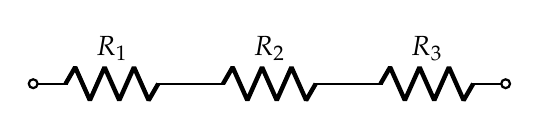
\begin{tikzpicture}
      \draw[thick](0,0) to[R=$R_1$,o-] (2,0) to[R=$R_2$] (4,0)
      to[R=$R_3$,-o] (6,0);
    \end{tikzpicture}
  \end{center}

  \vspace{.1in}The analysis for resistors in series is similar (but easier).
  From the current law, the current through each resistor is the same:

  \eq{-.2in}{I_1=I_2=I_3=\cdots=I}

  \vspace{-.15in}And the total voltage drop across all resistor is therefore:

  \eq{-.4in}{V=V_1+V_2+V_3+\cdot=I(R_1+R_2+R_3+\cdots)}
\end{frame}

\begin{frame}
  \frametitle{Resistors in Series}
  \frametitle{Equivalent Resistance}
  Again, through applying Ohm's Law and Kirchkoff's laws, we find that when
  resistors are connected in series: \textbf{the equivalent resistance of loads
    is the sum of the resistances of the individual loads.}

  \eq{-.2in}{
    \boxed{R_\mathrm{eq}=R_1 + R_2 + \cdots + R_N}
  }

  \begin{center}
    \begin{tabular}{l|c|l}
      \rowcolor{pink}
      \textbf{Quantity} & \textbf{Symbol} & \textbf{SI Unit} \\ \hline
      Equivalent resistance          & $R_\mathrm{eq}$ & \si{\ohm} (ohm) \\
      Resistance of individual loads & $R_{1,2,3,\cdots,N}$ & \si{\ohm} (ohm) \\
    \end{tabular}
  \end{center}
\end{frame}


\begin{frame}
  \frametitle{Example Problem (Simple)}
  A simple circuit analysis problem will involve one voltage source and
  resistors connected, some in parallel, and some in series. Below is a typical
  example:

  \vspace{.2in}
  \begin{columns}
    \column{.4\textwidth}
    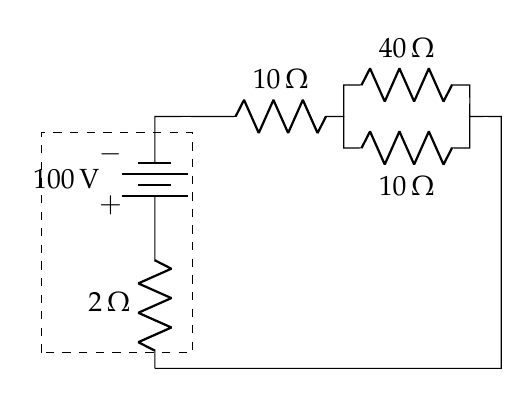
\begin{tikzpicture}[scale=.8,american voltages]
      \draw(0,0) to[R=2<\ohm>](0,2) to[battery=100<\volt>] (0,4) to[short]
      (1,4) to [R=10<\ohm>] (3,4)--(3,4.5) to[R=40<\ohm>] (5,4.5)
      to[short] (5,4) to[short] (5.5,4)--(5.5,0)--(0,0);
      \draw(3,4)--(3,3.5) to[R,l_=10<\ohm>] (5,3.5)--(5,4);
      \draw[dashed] (-1.8,0.25) rectangle(0.6,3.75);
    \end{tikzpicture}
    \column{.6\textwidth}
    Two \SI{10}{\ohm} resistors and a \SI{40}{\ohm} resistor are connected as
    shown to a \SI{100}{\volt} emf source with internal resistance
    \SI{2}{\ohm}. How much power is dissipated by the \SI{40}{\ohm} resistor?
    \begin{enumerate}[(A)]
    \item\SI{160}{\watt}
    \item\SI{40}{\watt}
    \item\SI{400}{\watt}
    \item\SI{5}{\watt}
    \item\SI{500}{\watt}
    \end{enumerate}
  \end{columns}
\end{frame}


\begin{frame}
  \frametitle{Tips for Solving ``Simple'' Circuit Problems}
  \begin{enumerate}
  \item Identify groups of resistors that are in parallel or in series, and
    find their equivalent resistance.
  \item Gradually reduce the entire circuit to one voltage source and one
    resistor.
  \item Using Ohm's law, find the current out of the battery.
  \item Uing Kirchkoff's laws, find the current through each of the resistors.
  \end{enumerate}
\end{frame}

\begin{frame}
  \frametitle{Circuits Aren't Always Simple}
  Some of these problems require you to solve a system of linear equations.
  The following is a simple example with two voltage sources:
  \begin{center}
    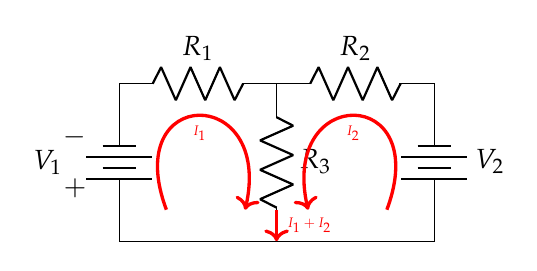
\begin{tikzpicture}[american voltages]
      \draw(0,0) to[battery=$V_1$](0,2) to[R=$R_1$](2,2) to[R=$R_3$](2,0)--(0,0);
      \draw(2,0)--(4,0) to[battery,l_=$V_2$](4,2) to[R,l_=$R_2$](2,2);
      \uncover<2->{
        \draw[very thick,red,->](2,0.4)--(2,0)
        node[midway,right]{\tiny $I_1+I_2$};
        \draw[very thick,red,->] (0.6,0.4)..controls (0,2) and (2,2)..(1.6,.4)
        node[midway,below]{\tiny $I_1$};
        \draw[very thick,red,->] (3.4,0.4)..controls (4,2) and (2,2)..(2.4,.4)
        node[midway,below]{\tiny $I_2$};
      }
    \end{tikzpicture}
  \end{center}
  \uncover<2->{
    In this case, we have to draw two loops of current.
  }
\end{frame}

\begin{frame}
  \frametitle{A More Difficult Example}
  \begin{columns}
    \column{.4\textwidth}
    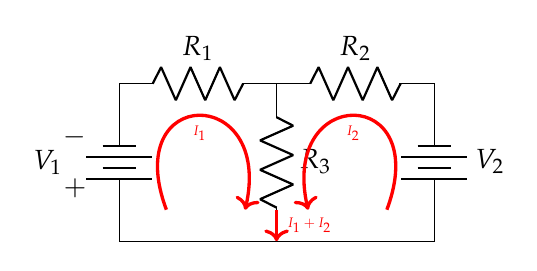
\begin{tikzpicture}[american voltages]
      \draw(0,0) to[battery=$V_1$](0,2) to[R=$R_1$](2,2)to[R=$R_3$](2,0)--(0,0);
      \draw(2,0)--(4,0) to[battery,l_=$V_2$](4,2) to[R,l_=$R_2$](2,2);
      \draw[very thick,red,->](2,0.4)--(2,0)
      node[midway,right]{\tiny $I_1+I_2$};
      \draw[very thick,red,->] (0.6,0.4)..controls (0,2) and (2,2)..(1.6,.4)
      node[midway,below]{\tiny $I_1$};
      \draw[very thick,red,->] (3.4,0.4)..controls (4,2) and (2,2)..(2.4,.4)
      node[midway,below]{\tiny $I_2$};
    \end{tikzpicture}
    \column{.6\textwidth}
    We split the circuit into two loops, and apply Kirchkoff's voltage in both:

    \vspace{-.4in}{\Large
      \begin{align*}
        V_1-I_1R_1-(I_1+I_2)R_3&=0\\
        V_2-I_2R_2-(I_1+I_2)R_3&=0
      \end{align*}
    }
  \end{columns}
  Two equations, two unknowns ($I_1$ and $I_2$). We can subtract (2) from (1),
  then solve for $I_1$ and $I_2$:

  \eq{-.4in}{
    I_1=\frac{V_1-I_2R_3}{R_1+R_3}
    \quad\quad
    I_2=
    \frac{\left[V_2-\frac{(V_1-V_2)R_3}{R_1}\right]}
         {\left[R_2+\frac{(R_1+R_2)R_3}{R_1}\right]}
  }

  (Try this at home as an exercise.)
\end{frame}





\section{Capacitors in Circuits}


\begin{frame}
  \frametitle{Capacitors in Parallel}

%  \begin{columns}
%    \column{.25\textwidth}
%    \begin{tikzpicture}[scale=1.2]
%      \fill[red!65!black](0,0) circle(0.07);
%      \draw[dashed,thick](0,0) circle(1.5);
%      \foreach \x in {0,...,13}{
%        \draw[red!65!black,thick,rotate=30*\x,->](0,0)--(0,1);
%      }
%      \draw[thick,->](0,1.5)--(0,2)
%      node[pos=1,above]{\footnotesize$\hat{\mb{n}}$};
%      \node[red!65!black] at (1.1,0) (E) {\footnotesize$\mb{E}$};
%    \end{tikzpicture}
%    \column{.75\textwidth}
%    By symmetry, electric field lines are radially outward from the charge, so
%    the integral reduces to:

  \eq{-.2in}{\boxed{C_\mathrm{eq}=C_1+C_2+\cdots+C_N}}

%    Since area of a sphere is $A=4\pi r^2$, we recover Coulomb's law:
%
%    \eq{-.3in}{ E=\frac{1}{4\pi\epsilon_0}\frac{q}{r^2}=\frac{kq}{r^2}}
%    
%    (In fact, it was through studying point charges that Gauss's law was
%    discovered, so it should not be a surprise that they agree.)
%  \end{columns}
\end{frame}


\begin{frame}
  \frametitle{Capacitors in Series}
%  In the homework questions this week, you will be asked to find the
%  electric field strength inside and outside of a few common configurations:
%  \begin{itemize}
%  \item Inside \& outside of a spherical shell of charge
%  \item Inside \& outside of a uniformly charged solid sphere
%  \item Near an infinite line charge
%  \item Inside \& outside an infinitely long solid cylinder of charge
%  \item Inside \& outside a cylindrical shell of charge
%  \end{itemize}
\end{frame}


\section{R-C Circuits}


\begin{frame}
  \frametitle{Circuits with Resistors and Capacitors}
%  \begin{columns}
%    \column{.25\textwidth}
%    \pic{1.3}{elec_gauss_figure9.jpg}
%    \column{.75\textwidth}
%    \begin{itemize}
%    \item Charge density (charge per unit area) $\sigma$
%    \item By symmetry, $\mb{E}$ must be perpendicular to the plane
%    \item Our Gaussian surface is a cylinder shown in the left with an area
%      $A$; the height of the cylinder is unimportant
%    \item We can see that nothing ``flows out'' of the side of the cylinder,
%      only at the ends.
%    \item The total flux is $\Phi=E(2A)$
%    \item The enclosed charge is $Q_\mathrm{encl}=\sigma A$.
%    \end{itemize}
%  \end{columns}
\end{frame}


\begin{frame}
  \frametitle{Discharging a capacitor}
%  \begin{columns}
%    \column{.3\textwidth}
%    \pic{1.25}{elec_gauss_figure9.jpg}
%    \column{.7\textwidth}
%    Gauss's law simplifies to:
%    
%    \eq{-.35in}{
%      \oint\mb{E}\cdot d\mb{A}=\frac{Q_\mathrm{encl}}{\epsilon_0}
%      \;\;\rightarrow\;\;
%      E(2A)=\frac{\sigma A}{\epsilon_0}
%    }
%
%    Solving for $E$, we get:
%
%    \eq{-.3in}{\boxed{E=\frac{\sigma}{2\epsilon_0}}}
%    \begin{itemize}
%    \item $E$ is a constant
%    \item Independent of distance from the plane
%    \item Both sides of the plane are the same
%    \end{itemize}
%  \end{columns}
\end{frame}



\begin{frame}
  \frametitle{Charging a Capacitor}
%  Remember being told that the electric field between two charged plates
%  is constant?
%
%  \begin{itemize}
%  \item Two plates, each producing an electric field pointing in the same
%    direction
%  \item The total electric field is twice the value that we found on the last
%    slide
%
%    \eq{-.1in}{\boxed{E=\frac{\sigma}{\epsilon_0}}}
%
%    which is what we already know!
%  \end{itemize}
\end{frame}



%\section{Capacitors}
%
%
%\begin{frame}
%  \frametitle{Capacitors}
%  \textbf{Capacitors} stores energy in a circuit. The
%  simplest form of a capacitor is a set of closely spaced parallel plates:
%
%  \vspace{-.3in}
%  \begin{center}
%    \pic{.5}{cap19.png}
%  \end{center}
%  
%  \vspace{-.15in}When the plates are connected to a battery, the battery
%  transfer charges to the plates until the potential difference (voltage) $V$
%  equals the battery terminals. This takes almost no time. After that, one
%  plate has charge $+Q$; the other has $-Q$.
%\end{frame}
%
%\begin{frame}
%  \frametitle{Parallel-Plate Capacitors}
%  Since we know what $E=\sigma/\epsilon_0$ between the plates, and the
%  relationship $E=V/d$, we can relate $V$ to the amount of charge $Q$ stored
%  between the plates:
%
%  \eq{-.3in}{ V=Ed=\frac{\sigma}{\epsilon_0}d=\frac{Qd}{\epsilon_0A}}
%
%  The ratio between charge $Q$ and voltage $V$ is defined as the
%  \textbf{capacitance} $C$:
%
%  \eq{-.1in}{
%    \boxed{C=\frac{Q}{V}}
%    \quad\quad
%    \text{\normalsize for parallel plates:}
%    \;\;
%    C=\frac{\epsilon_0A}{d}
%    \;\;\text{\normalsize (constant!)}
%  }
%\end{frame}
%
%
%\begin{frame}
%  \frametitle{Parallel-Plate Capacitors}
%
%  Capacitance $C$ is defined as the ratio between charge $Q$ ($+$ on one
%  plate; $-$ on the other) and potential difference (voltage) $V$:
%  
%  \eq{-.05in}{
%    \boxed{C=\frac{Q}{V}}
%  }
%  
%  \begin{center}
%    \begin{tabular}{l|c|l}
%      \rowcolor{pink}
%      \textbf{Quantity} & \textbf{Symbol} & \textbf{SI Unit} \\ \hline
%      Capacitance   & $C$   & \si{\farad} (farads)\\
%      Charge        & $Q$   & \si{\coulomb} (coulombs)\\
%      Voltage across the plates & $V$ & \si{\volt} (volts)
%    \end{tabular}
%  \end{center}
%
%\end{frame}
%
%\begin{frame}
%  \frametitle{Real Capacitors}
%  \begin{columns}
%    \column{.25\textwidth}
%    \pic{1.2}{Figure_20_05_05a.jpg}
%    \column{.75\textwidth}
%    \begin{itemize}
%    \item Parallel-plate capacitors are very common in electric circuits,
%      but a vacuum between the plates is not very effective
%    \item Instead, a \textbf{dielectric} (nonconducting) material is inserted
%      between the plates
%    \item When the plates are charged, the electric field of the plates
%      polarizes the dielectric.
%    \item The dielectric now produces an electric field that opposes the field
%      from the plates, therefore reduces the effective voltage, and increasing
%      the capacitance
%    \end{itemize}
%  \end{columns}
%\end{frame}
%
%
%\begin{frame}
%  \frametitle{Dielectric Constant}
%  \begin{columns}
%    \column{.65\textwidth}
%    If electric field without dielectric is $E_0$, then $E$ in the
%    dielectric is reduced by $\kappa$, the \textbf{dielectric constant}:
%
%    \eq{-.25in}{\boxed{E=\frac{E_0}{\kappa}}}
%
%    \vspace{-.1in}The capacitance in a dielectric is now amplified:
%
%    \eq{-.25in}{\boxed{C=\kappa C_0}}
%
%    \vspace{-.15in}We can also view the dielectric as something that
%    increases the effective permittivity:
%
%    \eq{-.3in}{\boxed{\epsilon=\kappa\epsilon_0}}
%
%    \column{.35\textwidth}
%    \begin{tabular}{l|l}
%      \rowcolor{pink}
%      \textbf{Material} & $\kappa$ \\ \hline
%      Air         & \num{1.00059} \\
%      Bakelite    & \num{4.9} \\
%      Pyrex glass & \num{5.6} \\
%      Neoprene    & \num{6.9} \\
%      Plexiglas  & \num{3.4} \\
%      Polystyrene & \num{2.55} \\
%      Water (\SI{20}{\celsius}) & \num{80} 
%    \end{tabular}
%    \end{columns}
%\end{frame}
%
%
%\begin{frame}
%  \frametitle{Storage of Electrical Energy}
%  \begin{center}
%    \pic{.45}{slide14.jpg}
%  \end{center}
%
%  \begin{itemize}
%  \item When charging up a capacitor, imagine positive charges moving from the
%    negatively charged plate to the positively charged plate
%  \item Initially neither plates are charged, so moving the first charge takes
%    very little work; as the electric field builds, more and more work needs
%    to be done
%  \end{itemize}
%\end{frame}
%
%\begin{frame}
%  \frametitle{Storage of Electrical Energy}
%
%  Starting from the beginning---when the plates aren't charged---if we move an
%  infinitesimally charge $dq$ across the plates, the infinitesimal work done
%  $dU$ is related to the capacitance:
%
%  \eq{-.3in}{dU=Vdq=\frac{q}{C}dq}
%
%  \vspace{-.1in}To fully charge the plates, the total work $U$ is the integral:
%
%  \eq{-.2in}{U=\int dU=\int_0^Q\frac{q}{C}dq=\frac{1}{2}\frac{Q^2}{C}}
%
%  There are different ways to express $U$ using definition of capacitance:
%
%  \eq{-.2in}{\boxed{U=\frac{1}{2}\frac{Q^2}{C}=\frac{1}{2}QV=\frac{1}{2}CV^2}}
%\end{frame}
\end{document}
